\documentclass[aspectratio=43]{beamer}

\usepackage[utf8]{inputenc}
\usepackage[russianb]{babel}
\usepackage{amssymb}
\usepackage{amsmath}
\usepackage{moreverb}

% flowcharts
\usepackage{tikz}
\usetikzlibrary{shapes,arrows,
	decorations.pathreplacing,decorations.pathmorphing}
	
% for tables
\usepackage{multirow}
\usepackage{hhline}
\usepackage{color, colortbl}

% include pictures
\usepackage{graphicx}
\DeclareGraphicsExtensions{.png}
\graphicspath{ {pics/} }	

\usetheme{default}
\usecolortheme{default} % \usecolortheme{dove} for print
\usefonttheme{professionalfonts}

\begin{document}

\begin{frame}
\begin{center}
ФГБОУ ВПО МГТУ «СТАНКИН»
 
\medskip
Факультет  информационных технологий и систем управления
Кафедра информационных систем

\medskip
Выпускная квалификационная работа
по направлению  230400.62 «Информационные системы и технологии»
\end{center}

\begin{block}{\centering{Разработка программной среды аналитического моделирования практико-ориентированных информационных систем}}
\end{block}

Студент группы ИДБ-11-01: Лакеев Р.Д. \\
Научный руководитель: д.т.н., проф. Климанов В.П.

\bigskip
\centerline{Москва, 2015 г.}
\end{frame}

\begin{frame}
\frametitle{Введение}

\begin{block}{Цель}
Анализ критериев времени и надёжности доставки информации в информационно-вычислительных сетях.
\end{block}

\begin{block}{Задачи}
\begin{enumerate}
	\item Изучение методики разработки моделей сетей.
	\item Разработка аналитических математических моделей ИВС.
	\item Разработка программы для вычисления стационарных и интегральных вероятностных характеристик заданной ИВС.
	\item Проведение модельного эксперимента.
\end{enumerate}
\end{block}
\end{frame}

\begin{frame}
\frametitle{Введение}

\begin{enumerate}
	\item  Составление уравнений баланса интенсивностей потоков.
	\item  Вычислеие коэффициентов передачи из уравнений баланса.
	\item  Вычисление стационарных вероятностно-временных характеристик (ВВХ) для каждого отдельного элемента СеМО.
	\item  Вычисиление интегральных ВВХ при взаимодействии двух любых абонентов сети.
	\item Вычисление плотностей распределения сообщений в самом коротком и длинном маршруте.
	\item Вычисления коэффициента структурной надёжности сети.
\end{enumerate}
\end{frame}

\begin{frame}

\begin{block}{Программная платформа}
Реализация выполнена на языке C\# и программной платформе Mono.
Mono --- кроссплатформенная реализация Microsoft .Net Framework с открытым исходным кодом.
Среда разработки --- MonoDevelop.
\end{block}
\end{frame}

\begin{frame}

\begin{block}{Исходные данные}
Исходными параметрами модели являются интенсивности обслуживающих узлов сети \( \mu_{i}^{m} \), интенсивности поступления сообщений из внешнего источника
\( \lambda_{i}^{m} \) и маршрутная матрица \( P^{m} \) для каждого входного потока \( m = \overline{1, F} \).

Интенсивности узлов сети \( \mu_{i}^{m} \) рассчитываются в соответствии с выбранной технологией Ethernet и длиной сообщения.
\end{block}
\end{frame}

\begin{frame}

\begin{tabular}{|p{0.22\textwidth}|p{0.22\textwidth}|p{0.22\textwidth}|p{0.22\textwidth}|}
	\hline Технология Ethernet & Битовая скорость & Длина кадра (байт) & Интенсивность \( \mu \) (кадр/мс) \\
	\hline \multirow{2}{*}{Fast Ethernet} 	& \multirow{2}{*}{100 Мбит/с} 	& 72 	& 148.800 \\
	\hhline{~~--}				  			& \multirow{2}{*}{}           	& 1526 	& 8.127 \\ 
	
	\hline \multirow{2}{*}{Gigabit Ethernet} 	& \multirow{2}{*}{1 Гбит/с} 		& 72 	& 1488.095 \\
	\hhline{~~--}				  			& \multirow{2}{*}{}           	& 1526 	& 81.274 \\ 
	
	\hline \multirow{2}{*}{10G Ethernet} 		& \multirow{2}{*}{10 Гбит/с} 	& 72 	& 14880.952 \\
	\hhline{~~--}				  			& \multirow{2}{*}{}           	& 1526 	& 812.744 \\ 
	
	\hline \multirow{2}{*}{40G Ethernet} 		& \multirow{2}{*}{40 Гбит/с} 	& 72 	& 59523.800 \\
	\hhline{~~--}				  			& \multirow{2}{*}{}           	& 1526 	& 3250.975 \\ 
	
	\hline \multirow{2}{*}{100G Ethernet} 	& \multirow{2}{*}{100 Гбит/с} 	& 72 	& 148809.524 \\
	\hhline{~~--}				  			& \multirow{2}{*}{}           	& 1526 	& 8127.438 \\
	\hline
\end{tabular}
\end{frame}

\begin{frame}[fragile]
\frametitle{Пример работы программы}
\framesubtitle{Входные данные}

\begin{tiny}
\begin{columns}
\column{.5\textwidth}
\begin{listing}{1}
<NetworkConfiguration Name="Full-mesh topology">
  <RoutingMatrix>
    <Row>0;		-;		-;		-;		-</Row>
    <Row>0.25;	0;		0.25;	0.25;	0.25</Row>
    <Row>0.25;	0.25;	0;		0.25;	0.25</Row>
    <Row>0.25;	0.25;	0.25;	0;		0.25</Row>
    <Row>0.25;	0.25;	0.25;	0.25;	0</Row>
  </RoutingMatrix>

  <Nodes Count="4">
    <Stream Index="1">
      <Lambda>860; 930; 670; 710</Lambda>
        <Mu>
          <Ethernet Type="_10G"
            FrameLength="128"/>
        </Mu>
      </Stream>\end{listing}

\column{.5\textwidth}
\begin{listing}{17}
      <Stream Index="2">
        <Lambda>161; 153; 170; 167</Lambda>
        <Mu>
          <Ethernet Type="_10G"
            FrameLength="1024"/>
        </Mu>
      </Stream>
  </Nodes>
</NetworkConfiguration>\end{listing}
\end{columns}
\end{tiny}
\end{frame}

\begin{frame}
\frametitle{Пример работы программы}
\framesubtitle{Результаты вычислений}

\begin{block}{Результаты вычисления уравнений баланса}
\begin{tabular}{|c|c|c|c|c|c|}
\hline Поток & Характ. & Узел 1 & Узел 2 & Узел 3 & Узел 4 \\
\hline \multirow{3}{*}{1} 	& \( e_{i} \) & 1.017035 & 1.034700 & 0.969085 & 0.979180 \\
\hhline{~-----} 				& \( \lambda_{i}^{'} \) & 3224.000 & 3280.000 & 3072.000 & 3104.000 \\
\hhline{~-----} 				& \( \rho_{i} \) & 0.361088 & 0.367360 & 0.344064 & 0.347648 \\

\hline \multirow{3}{*}{2} 	& \( e_{i} \) & 0.997849 & 0.988018 & 1.008909 & 1.005223 \\
\hhline{~-----} 				& \( \lambda_{i}^{'} \) & 649.600 & 643.200 & 656.800 & 654.400 \\
\hhline{~-----} 				& \( \rho_{i} \) & 0.538388 & 0.533084 & 0.544356 & 0.542367 \\
\hline
\end{tabular}
\end{block}
\end{frame}

\begin{frame}
\frametitle{Пример работы программы}
\framesubtitle{Результаты вычислений}

\begin{block}{Стационарные вероятностно-временные характеристики}
\begin{tabular}{|c|c|c|c|c|c|}
\hline Поток & Характ. & Узел 1 & Узел 2 & Узел 3 & Узел 4 \\
\hline \cellcolor{black} 	& \( W_{i} \) & 0.004841 & 0.004851 & 0.004389 & 0.004441 \\

\hline \multirow{3}{*}{1} 	& \( U_{i} \) & 0.004953 & 0.004963 & 0.004501 & 0.004553 \\
\hhline{~-----} 				& \( L_{i} \) & 15.608149 & 15.911909 & 13.482236 & 13.785019 \\
\hhline{~-----}				& \( N_{i} \) & 15.969237 & 16.279269 & 13.826300 & 14.132667 \\

\hline \multirow{3}{*}{2} 	& \( U_{i} \) & 0.005670 & 0.005680 & 0.005218 & 0.005270 \\
\hhline{~-----} 				& \( L_{i} \) & 3.144868 & 3.120287 & 2.882530 & 2.906223 \\
\hhline{~-----}				& \( N_{i} \) & 3.683256 & 3.653371 & 3.426886 & 3.448590 \\
\hline
\end{tabular}
\end{block}
\end{frame}

\begin{frame}
\frametitle{Пример работы программы}
\framesubtitle{Результаты вычислений}

\begin{columns}[t]
\column{.5\textwidth}
\begin{block}{Все маршруты между узлами 1 и 4}
\begin{tabular}{|c|c|}
\hline Маршрут & Вероятность \\
\hline \( 1 \rightarrow 4 \) & 0.615385 \\
\hline \( 1 \rightarrow 2 \rightarrow 4 \) & 0.153846\\
\hline \( 1 \rightarrow 3 \rightarrow 4 \) & 0.153846\\
\hline \( 1 \rightarrow 2 \rightarrow 3 \rightarrow 4 \) & 0.038462 \\
\hline \( 1 \rightarrow 3 \rightarrow 2 \rightarrow 4 \) & 0.038461 \\
\hline
\end{tabular}
\end{block}

\begin{block}{Коэффициент структурной надёжности сети}
5
\end{block}

\column{.5\textwidth}
\begin{block}{Интегральные ВВХ}
\begin{tabular}{|c|c|c|}
\hline Поток & Харат. & Значение \\
\hline \cellcolor{black}		& \( W \) & 0.011486 \\

\hline \multirow{3}{*}{1} 	& \( U \) & 0.011761 \\
\hhline{~--} 				& \( L \) & 36.550228 \\
\hhline{~--} 				& \( N \) & 37.426723 \\

\hline \multirow{3}{*}{2} 	& \( U \) & 0.013526 \\
\hhline{~--} 				& \( L \) & 7.472934 \\
\hhline{~--} 				& \( N \) & 8.800595 \\
\hline
\end{tabular}
\end{block}
\end{columns}
\end{frame}

\begin{frame}
\frametitle{Пример работы программы}
\framesubtitle{Плотности распределения количества сообщений}

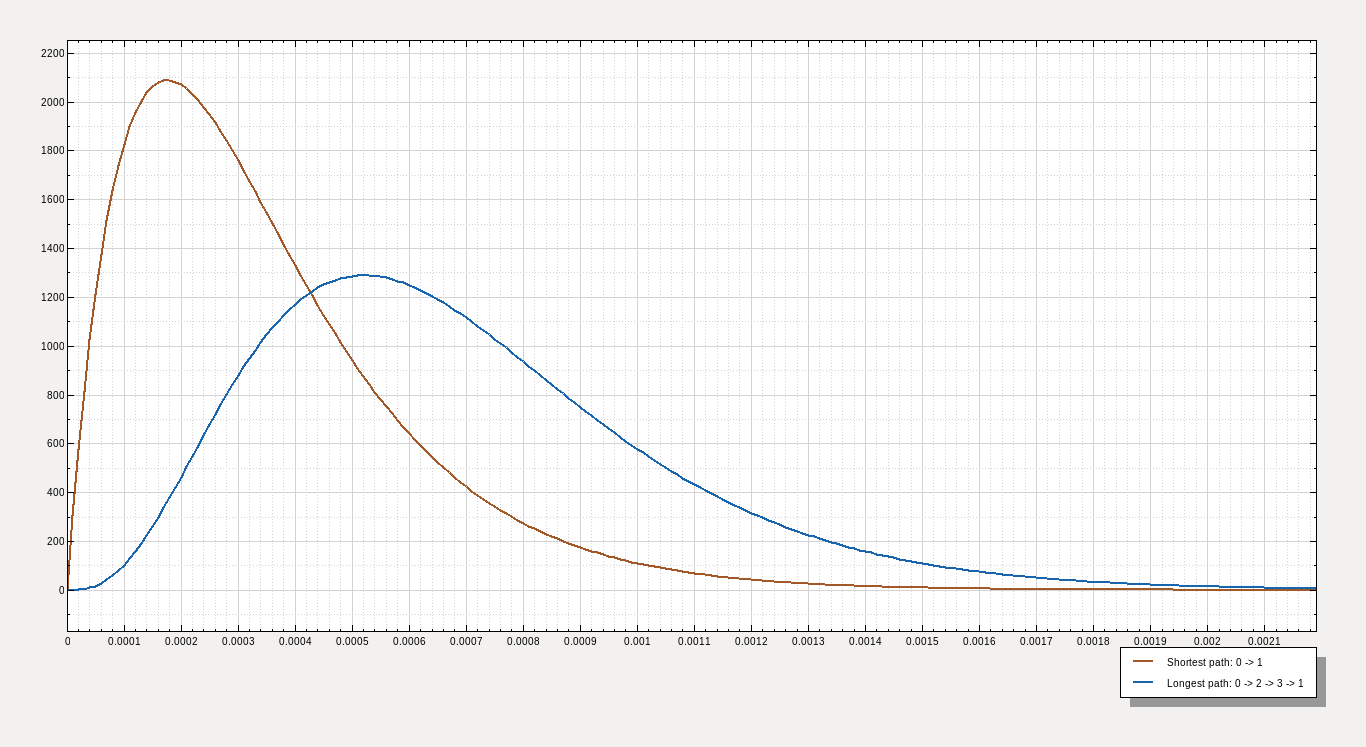
\includegraphics[width=.95\textwidth]{demo4_chart_2}
\end{frame}

\begin{frame}

\begin{block}{Модельный эксперимент}
Модельный эксперимент был проведён для следующих сетевых топологий:
\begin{enumerate}
	\item Шина	
	\item Звезда
	\item Кольцо
	\item Дерево
	\item Двухменая квадратная решётка
	\item Двухмерная треугольная решётка
	\item Трёхмерная квадратная решётся
	\item Пирамидальная топология	
	\item Полносвязная топология
\end{enumerate}
\end{block}
\end{frame}

\begin{frame}

\begin{tabular}{|p{0.22\textwidth}|p{0.22\textwidth}|p{0.22\textwidth}|p{0.22\textwidth}|}
	\hline Топология & Среднее время в маршруте (мс) & Коэффициент структурной надёжности & Количество связей \\
	\hline Шина  & 0.153211 & 1 & 9 \\
	\hline Звезда & 0.055320 & 1 & 9 \\
	\hline Кольцо & 0.014307 & 1 & 10 \\
	\hline Дерево & 0.064059 & 1 & 9 \\
	\hline Двухменая квадратная & 0.082925 & 4.844444 & 24 \\
	\hline Двухмерная треугольная & 0.089373 & 50.733333 & 18 \\
	\hline Трёхмерная квадратная & 0.069486 & 24.2 & 15 \\
	\hline Пирамидальная топология & 0.008404 & 503.522222 & 24 \\
	\hline Полносвязная топология & 0.013876 & 109601 & 45 \\
	\hline
	\end{tabular}
\end{frame}

\begin{frame}
\frametitle{Заключение}

В дипломной работе выполнено следующее:	
\begin{enumerate}
	\item Изучена методика построения моделей информационно- \\ вычислительных сетей.
	 
	\item Разработанна программа, автоматизирующая вычисления стационарных и интегральных вероятностно-временных характеристик, плотностей распределения сообщений в маршрутах сети и среднего количества маршрутов между любыми двумя узлами сети на основе заданной модели сети.
	
	\item Разработаны модели сетей с раными топологиями и с помощью разработанной программы проведён модельный эксперимент по их сравнению по времени и надёжности доставки сообщений.
\end{enumerate}
\end{frame}

\end{document}